
\documentclass{article}
\usepackage[a4paper]{geometry}
\usepackage{color}              % Controle das cores
\usepackage[utf8]{inputenc}
\usepackage[T1]{fontenc}
\usepackage[portuguese]{babel}
\usepackage{amsmath} % Permite diagramação matemática avançada
\usepackage{relsize}
\PassOptionsToPackage{hyphens}{url}\usepackage{hyperref} % Permite adicionar url's clicáveis
\usepackage{amssymb}
\usepackage{authblk}
\usepackage{tikz}
\usepackage{subfig}
\usepackage{float}
\usepackage{xcolor,colortbl}



\usetikzlibrary{matrix}

\DeclareMathOperator{\BigO}{O}

% Configura a exibição de urls
\hypersetup{
	colorlinks = true,
	urlcolor   = blue,
	linkcolor  = blue,
	citecolor  = black
}

\newenvironment{varalgorithm}[1]
{\algorithm\renewcommand{\thealgorithm}{#1}}
{\endalgorithm}



\title {\vspace{-3cm}EP 2 - Relatório}
\author{Felipe Constantino de Oliveira}
\affil{%
	MAC0417/5768 - Visão e Processamento de Imagens - IME-USP
}
\date{}
% ----
% Início do documento
% ----
\begin{document}
	
	\maketitle

	\section{Introdução}
	
	Este trabalho contém arquivos $.py$ e foi utilizada a seguinte configuração:
	\begin{itemize}
		\item Python 2.7
		\item OpenCV 3.4.1
		\item Numpy 1.14.3
		\item Matplotlib 2.1.2
		\item Scipy 1.1.0
	\end{itemize}
	
	\section{Problema 1}

	O primeiro desafio era utilizar os conceitos de Fourier para eliminar o ruído periódico na imagem do leopardo abaixo:
	
	\begin{figure}[H]
		\centering
		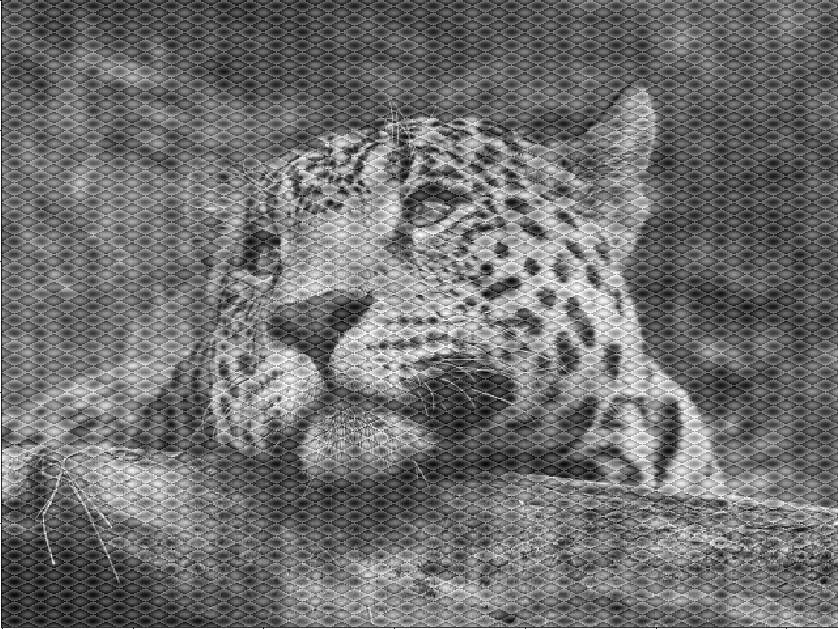
\includegraphics[scale=0.3]{images/1_original.png}
		\caption{Imagem com Ruído periódico} 
	\end{figure}

	Para isso, vamos analisar o espectro em Fourier. Nota-se pequenos pontos (alguns circulados em vermelho para facilitar a observação) que parecem estar afetando a qualidade da imagem. Podemos também aplicar uma limiarização para facilitar a visualização conforme imagens abaixo:
		
	\begin{figure}[H]
		\centering
		\subfloat[]{{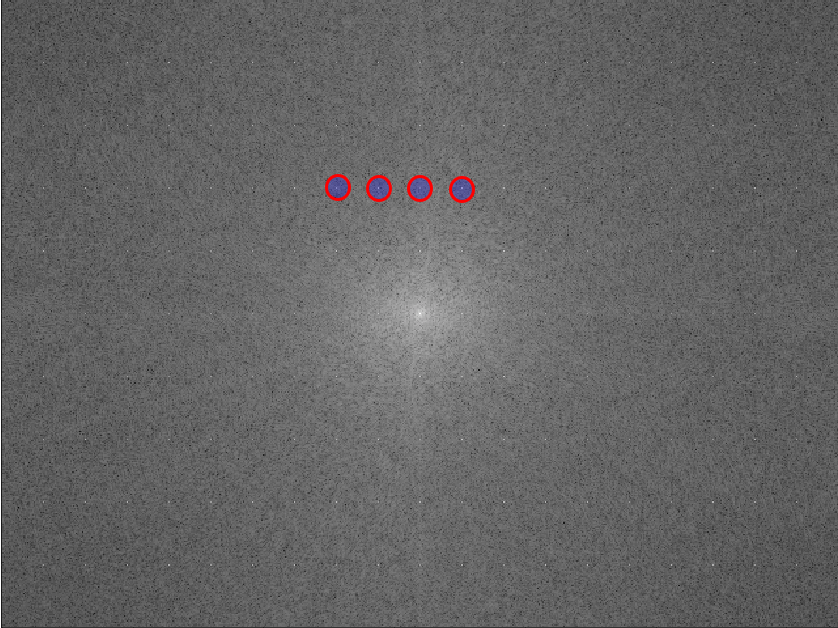
\includegraphics[scale=0.35]{images/1_spectrum.png} }}%
		\qquad
		\subfloat[]{{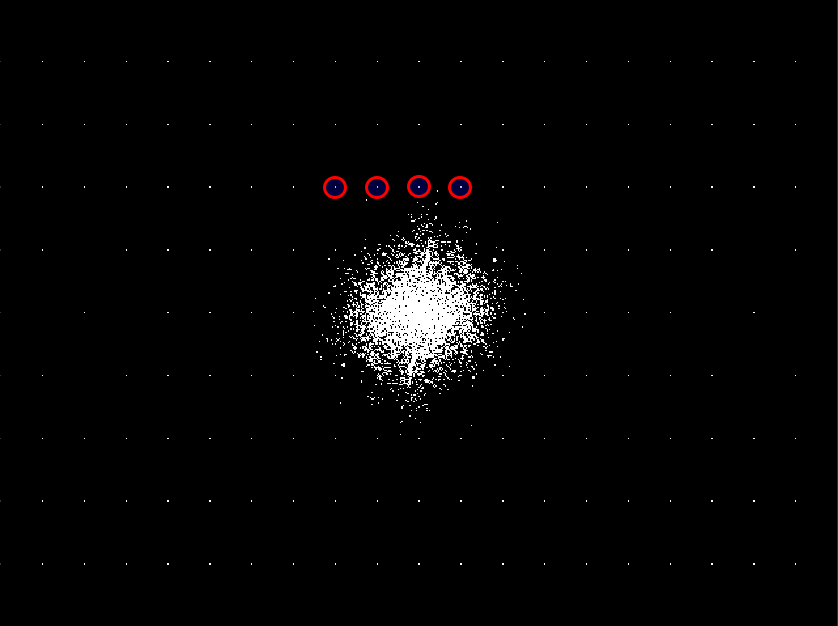
\includegraphics[scale=0.35]{images/1_spectrum_threshold.png} }}%
		\caption{Figura (a) contém o espectro e (b) com threshold de 60\%} 
	\end{figure}
	
	Além disso, podemos comparar o espectro em sua parte real e imaginária. Neste ponto é importante notar que existem tais pontos somente na parte real. 
	
	\begin{figure}[H]
		\centering
		\subfloat[]{{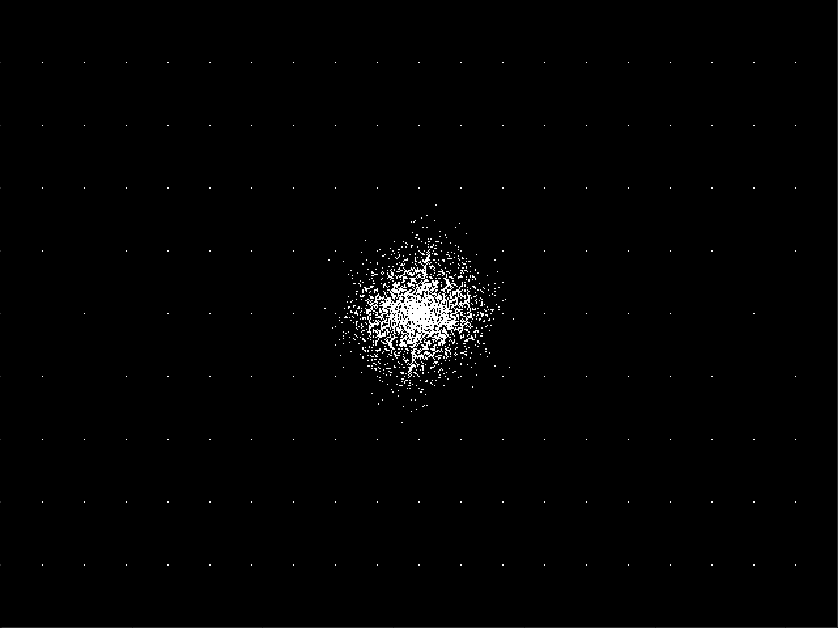
\includegraphics[scale=0.3]{images/1_spectrum_real.png} }}%
		\qquad
		\subfloat[]{{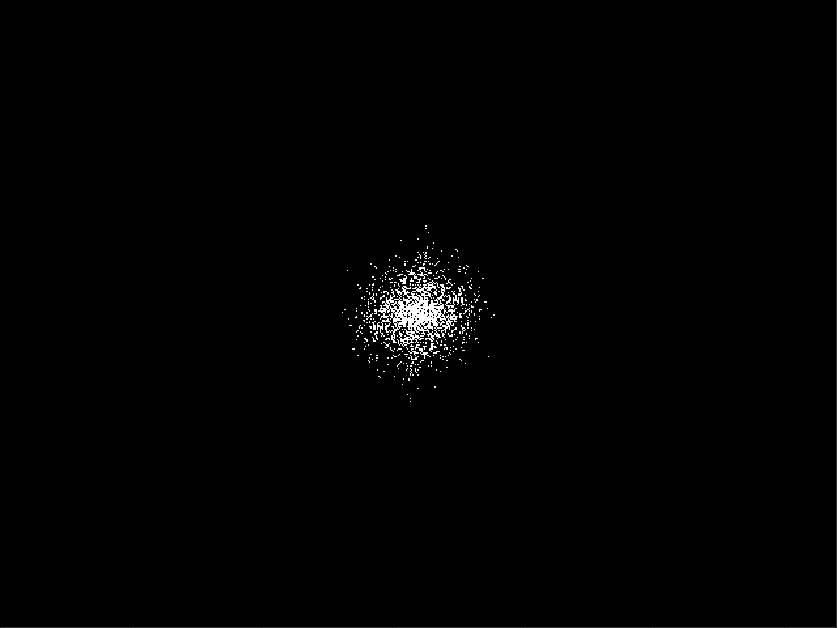
\includegraphics[scale=0.3]{images/1_spectrum_imag.png} }}%
		\caption{(a) Spectrum com threshold da parte real e (b) Spectrum com threshold da parte imaginária} 
	\end{figure}
	
	Como visto em aula e atividades do curso, pontos com valores acima do comum longe do centro podem ser ruído no domínio da imagem. Porém, como demonstrado acima e explorado com diversos thresholds, somente é possível observar tais pontos na parte real do espectro de Fourier e portanto, nos concentraremos em remover tais pontos nesta parte.
	
	Para remover os pontos que geram o ruído periódico, o algoritmo precisa de 3 parâmetros: (1) o espectro, (2) Um valor $s$ para o tamanho de um lado ímpar de um kernel quadrado ($k = s\times s$) e (3) um valor $t$ (chamado de código como $multiply\_factor$) que é um limiar de aceitação, onde $t > 1$.
	
	O algoritmo compara o valor absoluto do centro do kernel com os valores absolutos de seus vizinhos dado o kernel $k$. Se o pixel no centro do kernel é maior que todos os seus vizinhos vezes o limiar $t$, o novo valor do centro é a média entre os vizinhos.
	
	Na prática, alguns testes foram feitos e o melhor foi utilização de uma janela $5 \times 5$ onde $m=2$, ou seja, o valor do centro é pelo menos 2 vezes maior que valor máximo de seus vizinhos. Como resultado, temos a imagem (b) abaixo:
	
	\begin{figure}[H]
		\centering
		\subfloat[]{{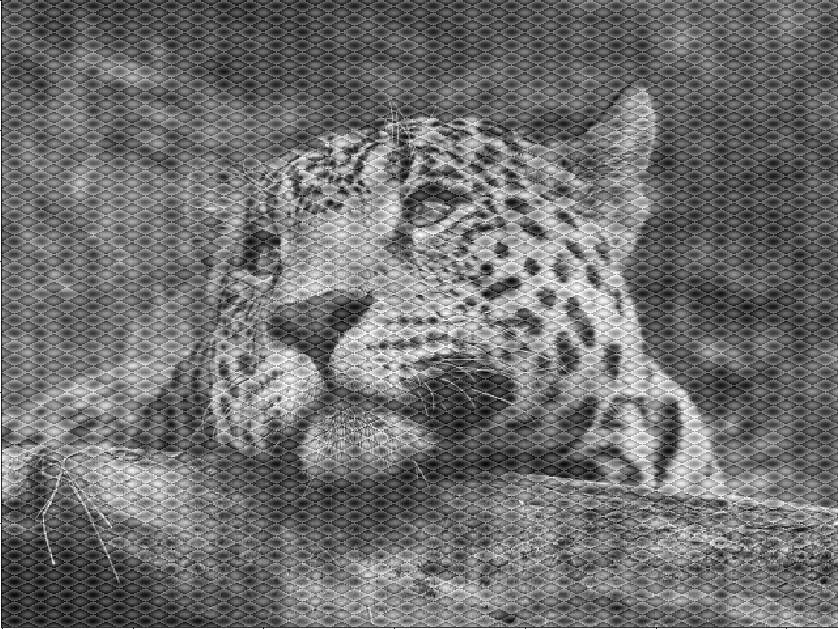
\includegraphics[scale=0.2]{images/1_original.png} }}%
		\qquad
		\subfloat[]{{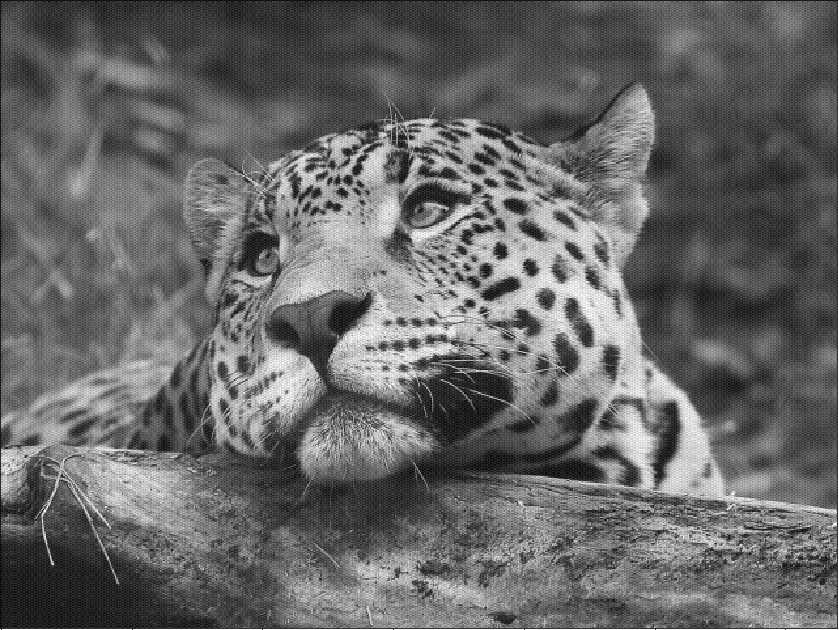
\includegraphics[scale=0.2]{images/1_output.png} }}%
		\caption{Figura (a) imagem de entrada (b) imagem de saída.} 
		
	\end{figure}
	
	
	\section{Problema 2}
	
	O problema número 2 também tinha como objetivo restaurar uma imagem corrompida, só que desta vez com um ruído impulsivo, resultando em diversas regiões pretas na imagem. 
	
	Para restaurar, foi pedido que se utilizasse o atributo área das bacias da Max-tree, no entanto como os ruídos a serem removidos são pretos, é necessário utilizar a Min-tree (dual da Max-tree) ou pode-se complementar a imagem e utilizar a Max-tree. Como estamos utilizando na matéria o \textit{siamxt Toolbox}, que só trabalha com Max-tree a segunda opção parece mais adequada.
	
	A figura 5 explora os resultados variando os valores do atributo de área. Como os ruídos são bem pequenos, ou seja, possuem poucos pixels conexos, um atributo de área pequeno já é o suficiente. 
	
	\begin{figure}[H]
		\centering
		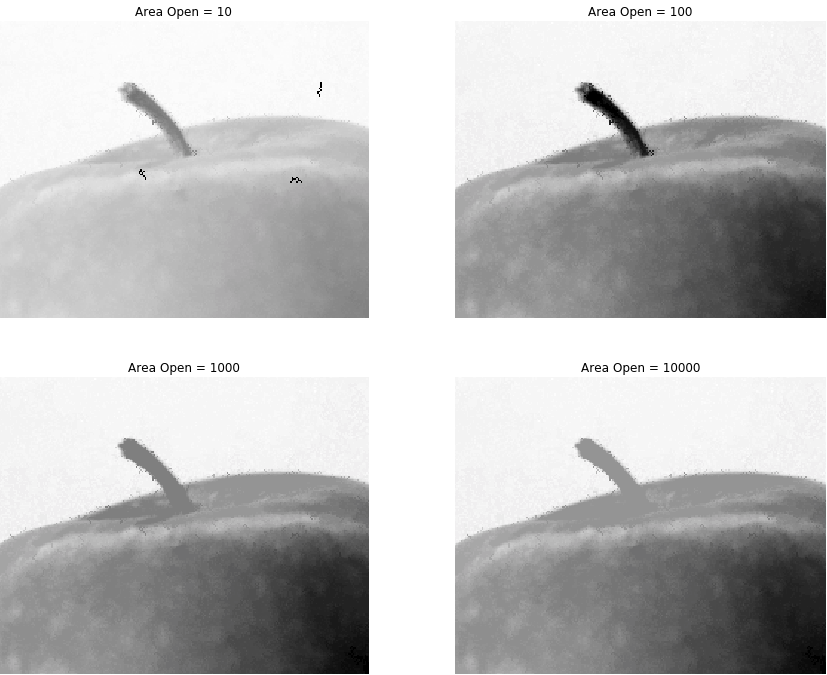
\includegraphics[scale=0.5]{images/2_maca_1.png}
		\caption{Detalhes da maçã após diversas podas com valores diferentes do atributo área}
	\end{figure}

	
	Podemos ver que com o atributo área = 10, temos uma boa quantidade de ruído eliminado. Porém ainda sobraram alguns grandes. Quando utilizamos uma pode com valor do atributo área muito grande como 1000 já acabamos afetando a imagem. Veja que o talo da maçã começou a perder o verdadeiro contraste. Além disso, se exageramos, como no exemplo utilizando 10000, além do talo, outros componentes da maçã acabam sendo prejudicados.
	
	Como o valor 100 pareceu adequado durante os testes, a imagem resultante após a aplicação da poda por área = 100 é a seguinte:
	
	\begin{figure}[H]
		\centering
		\subfloat[]{{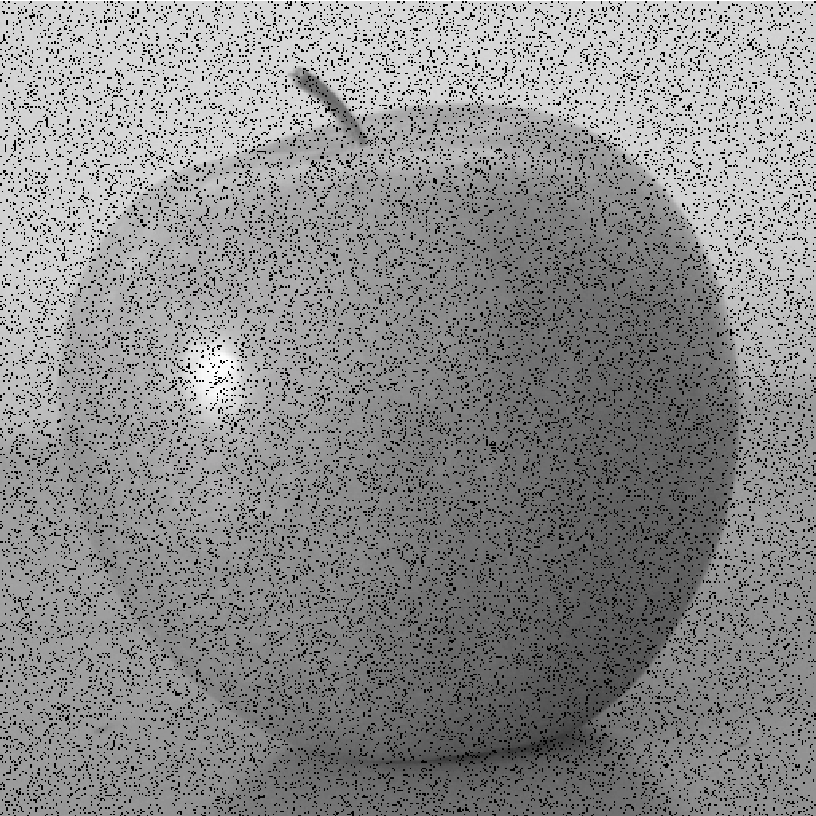
\includegraphics[scale=0.22]{images/2_maca_original.png} }}%
		\qquad
		\subfloat[]{{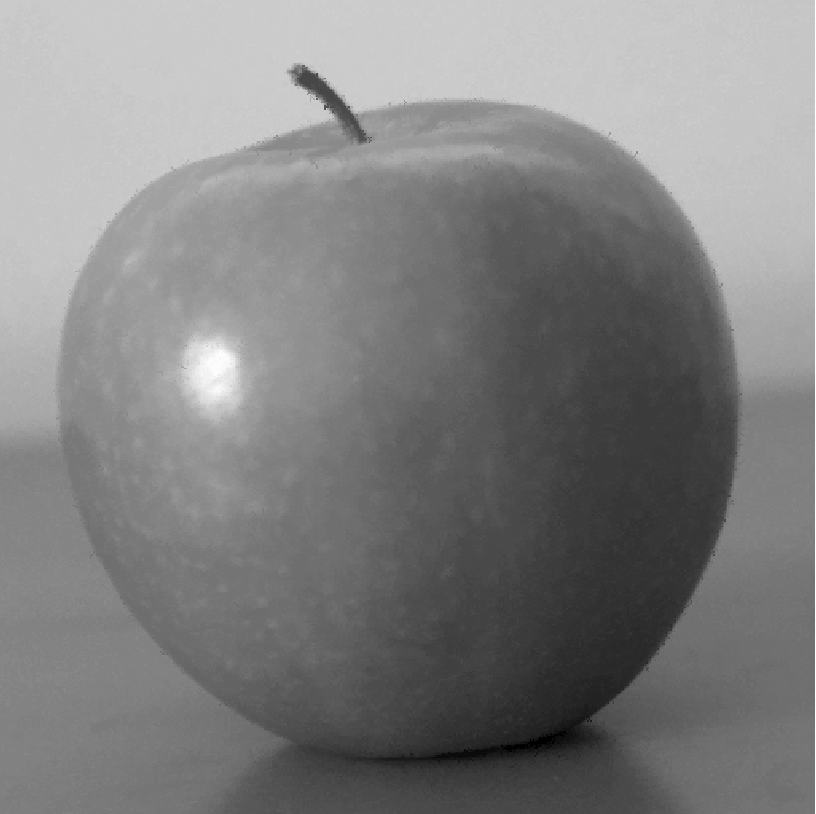
\includegraphics[scale=0.22]{images/2_maca_recuperada.png} }}%
		\caption{Figura (a) imagem de entrada (b) imagem de saída.} 
		
	\end{figure}
	
	
	\section{Problema 3}	
	
	O problema 3 tem como objetivo segmentar o joelho utilizando watershed. Só que para isso, acaba-se utilizando diversos conceitos apresentados na matéria a qual detalharemos a seguir.
	
	\subsection{Cálculo do Gradiente Morfológico}	
	
	Em morfologia matemática, Seja uma imagem em escala de cinza $I$ e um kernel $k$, Gradiente Morfológico é a diferença entre a dilatação e a erosão desta imagem, ou seja, $G(I) = (I \oplus k) - (I \ominus k)$.
	
	Conforme pedido pelo exercício, utilizaremos um disco de raio unitário como kernel, conforme demonstrado na Figura 7. 
	A aplicação do gradiente morfológico resulta na Figura 8.
	
	\begin{figure}[H]
		\centering
		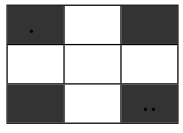
\includegraphics[scale=0.4]{images/3_disco.png}
		\caption{Disco de raio unitário} 
		
	\end{figure}
	
	
	\begin{figure}[H]
		\centering
		\subfloat[]{{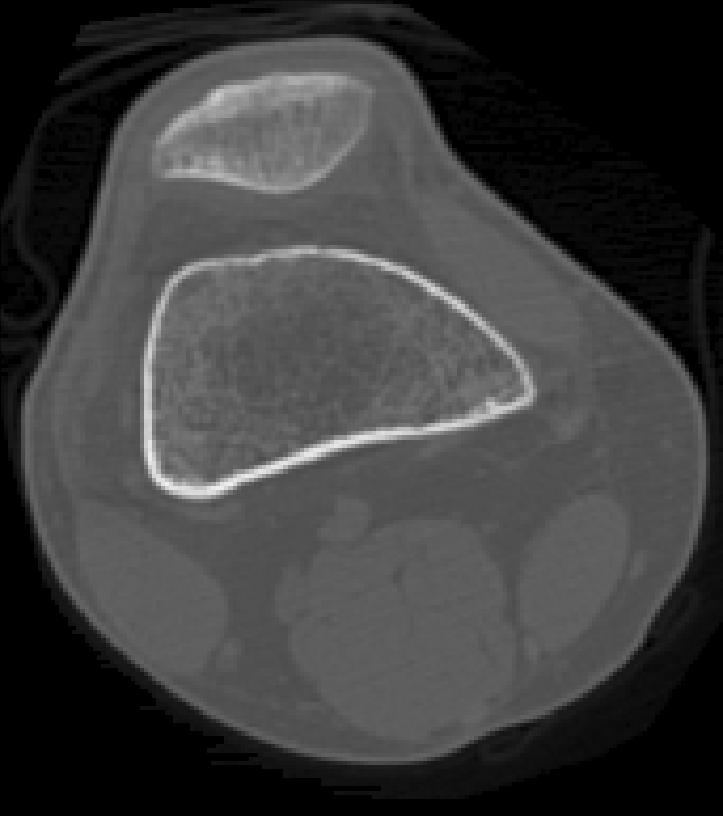
\includegraphics[scale=0.25]{images/3_original.png} }}%
		\qquad
		\subfloat[]{{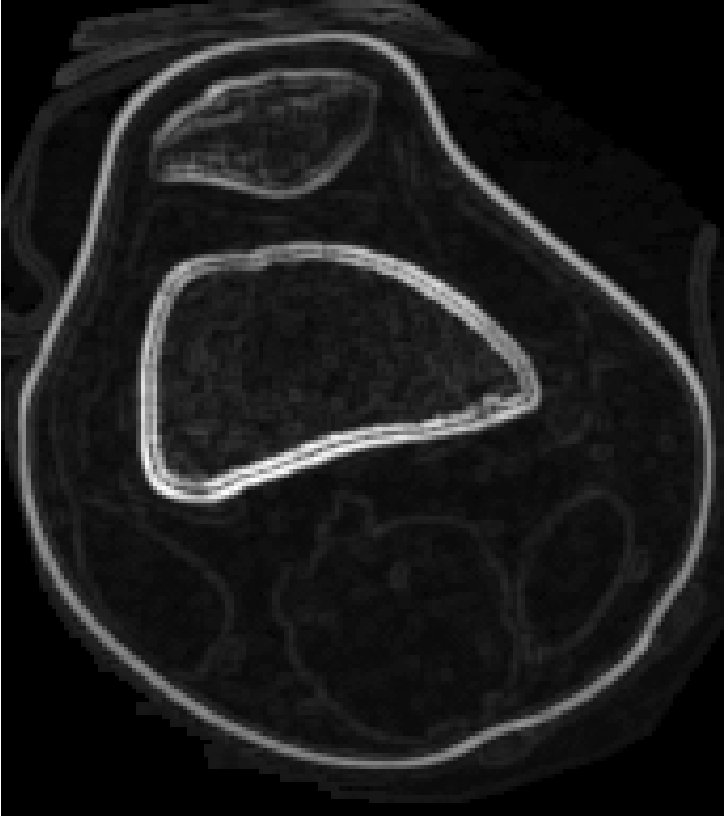
\includegraphics[scale=0.25]{images/3_gradiente.png} }}%
		\caption{Figura (a) imagem de entrada (b) imagem de saída.} 
		
	\end{figure}
	
	\subsection{Filtro das 8 bacias e Marcadores}	
		
	Agora precisamos aplicar um filtro em cima do resultado do gradiente morfológico. Similarmente ao problema 2, foi necessário complementar a imagem e utilizar a Max-tree, conservando as 8 folhas da Max-tree com a imagem complementada de acordo com o atributo calculado \textit{volume}. 
	
	Como resultado, tivemos outra imagem muito parecida com a do gradiente só que filtrada. Após isso, novamente calculamos a Max-tree da imagem resultante do passo anterior e dessa vez selecionamos somente as folhas. Como resultado, temos as 8 menores bacias da imagem.
	
	Estas bacias serão utilizadas como marcadores para o watershed. Para isso, foi necessário rotular cada um dos componentes conexos resultantes com uma cor, conforme imagem (a) abaixo. Após isso, rodamos o algoritmo de watershed, resultando na imagem (b) abaixo
	
	\begin{figure}[H]
		\centering
		\subfloat[]{{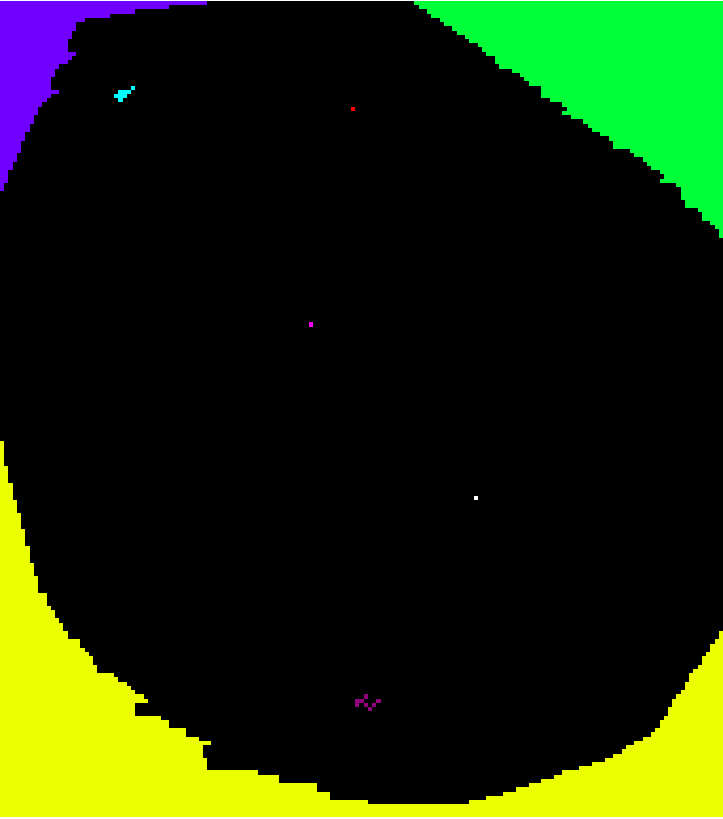
\includegraphics[scale=0.25]{images/3_pontos.png} }}%
		\qquad
		\subfloat[]{{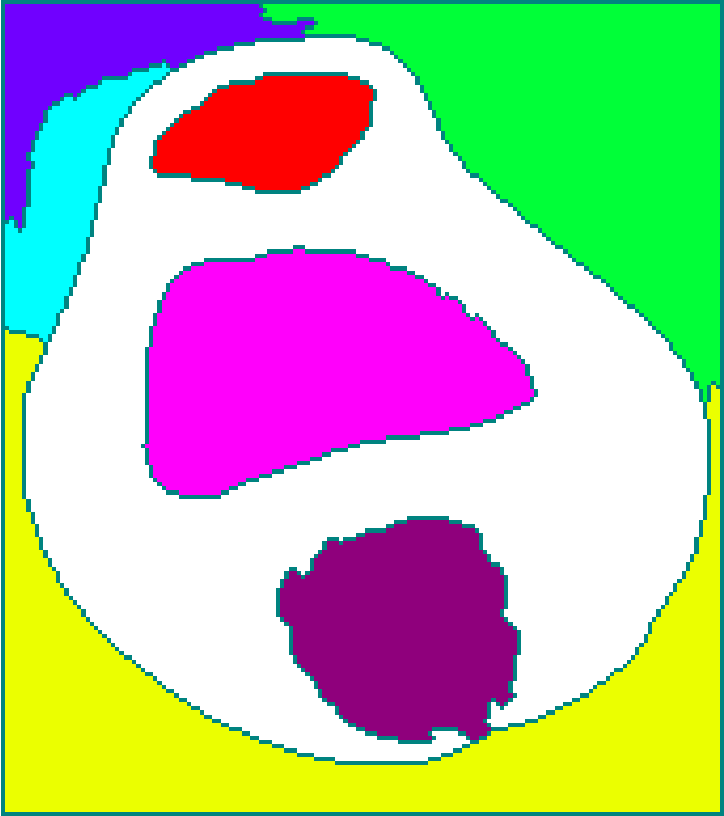
\includegraphics[scale=0.25]{images/3_resultado.png} }}%
		\caption{Figura (a) imagem de entrada (b) imagem de saída.} 
		
	\end{figure}
	

	\section{Problema 4}
	
	O problema 4 é um desafio de conseguir selecionar os caracteres alfanuméricos da melhor forma possível.
	
	Como primeiro passo, foi necessário utilizar filtros morfológicos para remover os fios de cabelo. O filtro com melhor resultado foi um fechamento de um elemento estruturante $5 \times 5$ circular, conforme ilustração abaixo:
	
	\begin{figure}[H]
		\centering
		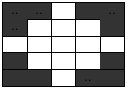
\includegraphics[scale=0.7]{images/4_struct.png}
		\caption{Elemento estruturante circular $5 \times 5$}
	\end{figure}
	
	A motivação por ele ser circular é tentar pegar a ondulação do cabelo, porém mantendo o aspecto arredondado das letras, Como resultado ainda tivemos alguns cabelos, principalmente aqueles que tiveram ficaram com sobra, resultando em um fio um pouco mais alongado
	
	\begin{figure}[H]
		\centering
		\subfloat[]{{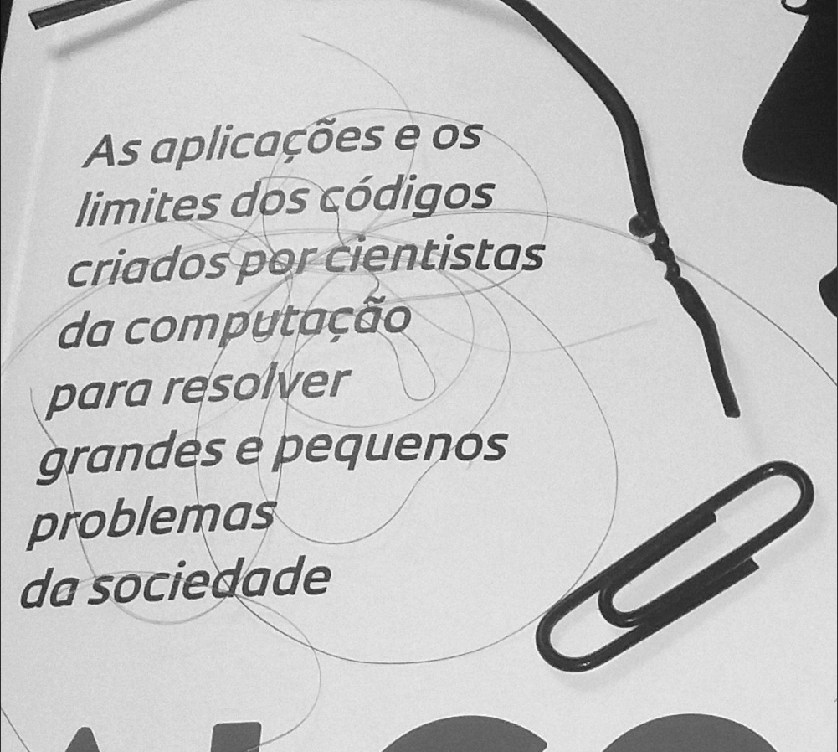
\includegraphics[scale=0.21]{images/4_original.png} }}%
		\qquad
		\subfloat[]{{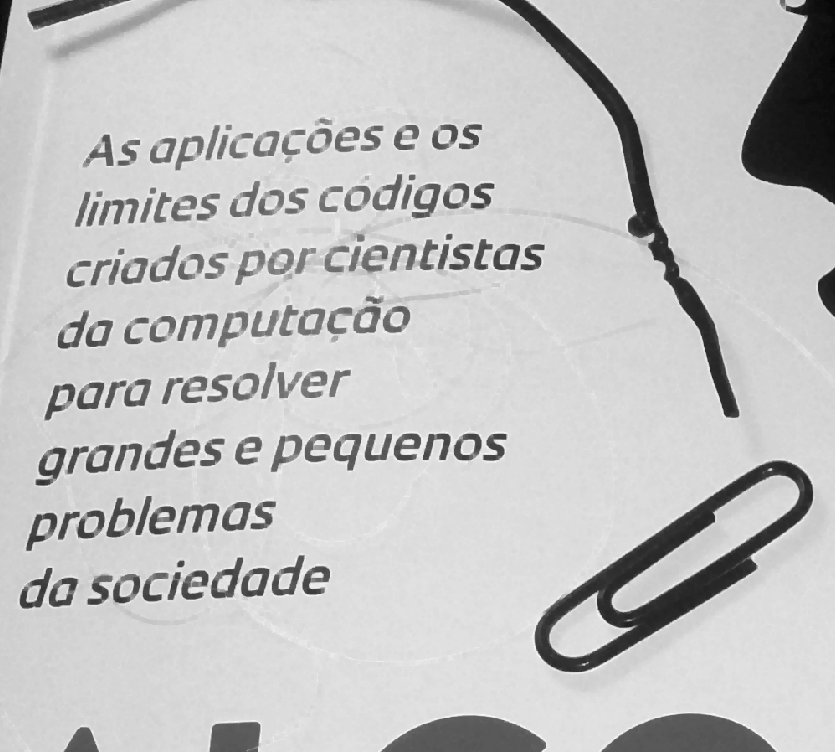
\includegraphics[scale=0.21]{images/4_removendo_cabelo.png} }}%
		\caption{Figura (a) imagem de entrada (b) imagem de saída.} 
	\end{figure}
	
	Após este filtro, o objetivo era conseguir retirar as letras da revista. Utilizou-se diversos filtros detalhados abaixo:
	
	\begin{itemize}
		\item Largura e altura mínimas e máximas da Bounding-box: A bounding-box, ou caixa delimitadora, é uma boa forma de eliminar letras que não possuem um certo aspecto. O filtro foi pensado levando-se em consideração diferenças por exemplo entre a letra ``I'' e a letra ``m''. Veja que elas possuem aspectos bem diferentes: o ``I'' tem altura grande, porém largura pequena, Já o ``m'' possui uma boa largura mas não muita altura.
		\item Razão de retangularidade mínima: tem por objetivo encontrar qual a porcentagem de preenchimento dentro da bounding-box, sendo assim possível eliminar o restante dos cabelos finos, já que eles provavelmente geraram uma caixa delimitadora mínima grande porém utilizando muito pouco seu preenchimento
		\item Altura mínima: A altura remove ruídos indesejados da imagem, removendo componentes isolados com padrão de brilho fora do esperado.
	\end{itemize}
	
	Como resultado dos filtros acima, pudemos gerar a imagem abaixo
	
	\begin{figure}[H]
		\centering
		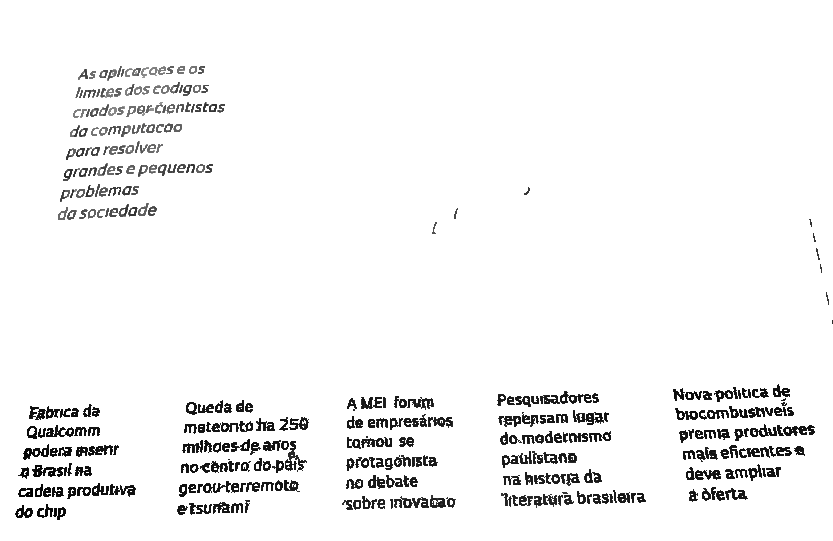
\includegraphics[scale=0.5]{images/4_resultado.png}
		\caption{Resultado após filtros na Max-tree}
	\end{figure}
	
\end{document}



